\section{Logistic Regression}
In logistic regression, the result of the prediction function $h(x)$ is between $0$ and $1$. This allows this value to also be considered a probability, making it ideal for classification tasks.
\begin{equation} \tag{Prediction Function}
    h_\theta(x) = g(\theta^Tx)
\end{equation}
Where:
\begin{equation} \tag*{}
    g(z) = \cfrac{1}{1+e^{-z}}
\end{equation}
The graphical representation is a sigmoid:
\begin{center}
    \begin{tabular}{c}
        \\ 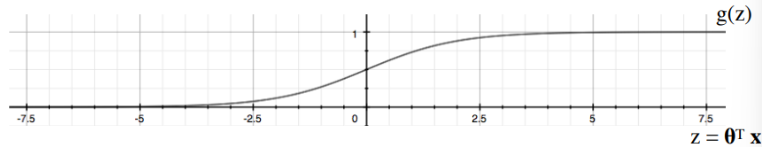
\includegraphics[width=0.9\textwidth]{images/LogisticRegression1.png} \\ \\
    \end{tabular}
\end{center}
This function can "flatten" or "widen", depending on the values within $\theta$, going to favor one class over another thereby succeeding in more accurately approximating a function that can divide the plane between classes.
\begin{equation} \tag*{}
    h_\theta(x) = \cfrac{1}{1+e^{-(\theta_0+\theta_1x)}}
\end{equation}
\begin{center}
    \begin{tabular}{c}
        \\ 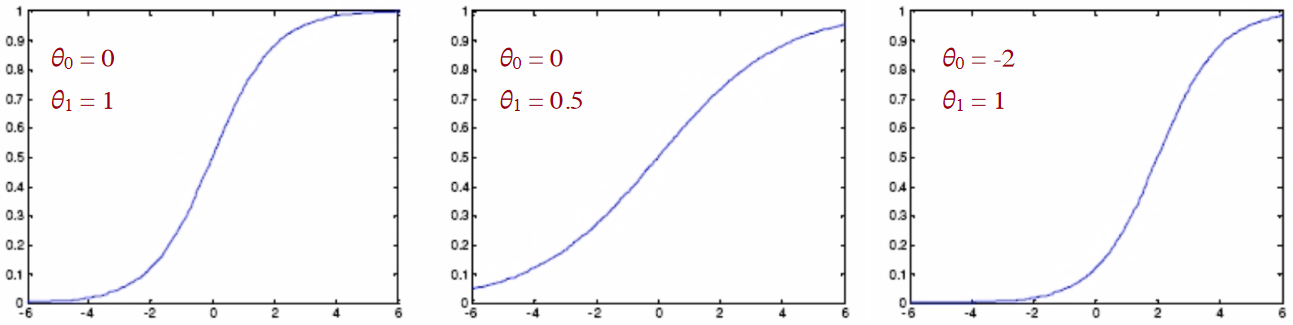
\includegraphics[width=0.9\textwidth]{images/LogisticRegression2.png}
    \end{tabular}
\end{center}

\subsection{Probabilistic Interpretation}
Logistic regression benefits from the marginalization property, so:
\begin{equation} \tag*{}
    h_\theta(x) = P(y=1|x;\theta)
\end{equation}
where $P(y=1|x;\theta)$ denotes the probability that $y=1$ given an input $x$, then:
\begin{equation} \tag*{}
    P(y=1|x;\theta) + P(y=0|x;\theta) = 1
\end{equation}
\newpage